\chapter{Thiết kế hệ thống}

% ============================================================
\reportsection{5.1 Hệ thống phần cứng}
% ============================================================

Kiến trúc phần cứng của đề tài được xây dựng theo mô hình tối giản nhưng đầy đủ
để thể hiện một mạng CAN thử nghiệm có khả năng sinh tấn công và phát hiện bất
thường. Mỗi nút CAN gồm một vi điều khiển ESP32 kết hợp với module thu phát CAN
TJA1050. Máy tính đóng vai trò điều khiển và giám sát, kết nối với ESP32 qua cổng
USB--UART; ứng dụng web trên máy tính không tham gia trực tiếp vào bus vật lý mà
gửi lệnh và nhận log phản hồi theo thời gian thực.

% ----------------------------------------------------------
\reportsubsection{5.1.1 ESP32}
% ----------------------------------------------------------

ESP32 đảm nhận toàn bộ phần xử lý điều khiển của nút. Firmware được nạp qua
PlatformIO với framework Arduino. Trong quá trình khởi động, ESP32 mở cổng UART
ở tốc độ 115.200 bps để phục vụ terminal và ghi log, đồng thời khởi tạo bộ điều
khiển CAN ở tốc độ 500 kbps.


\begin{table}[H]
\centering
\begin{tabular}{|>{\raggedright\arraybackslash}p{5cm}|>{\raggedright\arraybackslash}p{3cm}|>{\raggedright\arraybackslash}p{5.5cm}|}
\hline
\textbf{Tham số} & \textbf{Giá trị} & \textbf{Ghi chú} \\ \hline
Tốc độ CAN & 500 kbps & Phù hợp cho mô hình thử nghiệm \\ \hline
Chân TX CAN & GPIO 26 & Kết nối tới TXD của transceiver \\ \hline
Chân RX CAN & GPIO 27 & Kết nối tới RXD của transceiver \\ \hline
Tốc độ UART & 115.200 bps & Terminal và ghi log \\ \hline
Bảo vệ bộ đếm & Bật & Byte cuối mỗi khung là số thứ tự \\ \hline
Kích thước payload tối đa & 7 byte & Byte thứ 8 dành cho bộ đếm \\ \hline
Số ID theo dõi đồng thời & 16 & Giới hạn bộ nhớ của cấu trúc tracker \\ \hline
\end{tabular}
\caption{Cấu hình mặc định của firmware ESP32}
\end{table}

Vòng lặp chính của chương trình thực hiện tuần hoàn năm công việc: đọc lệnh từ
UART, thăm dò khung CAN mới từ bus, cập nhật các tác vụ tấn công định kỳ, điều
khiển LED báo hoạt động và phục vụ dấu nhắc terminal. Nhờ cách tổ chức vòng lặp
đơn luồng này, ESP32 vừa đóng vai trò nút truyền thông CAN vừa là bộ xử lý cục
bộ cho các thuật toán phát hiện xâm nhập.

% ----------------------------------------------------------
\reportsubsection{5.1.2 Module CAN TJA1050}
% ----------------------------------------------------------

TJA1050 là IC thu phát CAN của NXP Semiconductors, đảm nhận lớp vật lý theo chuẩn
ISO 11898-2. Trong mô hình của đề tài, TJA1050 thường được tích hợp sẵn trên một
board nhỏ có kèm điện trở kéo và tụ lọc. Phần tử này nhận tín hiệu logic từ GPIO
của ESP32, biến đổi thành cặp tín hiệu vi sai CANH/CANL và ngược lại. Các thông
số kỹ thuật chính được trình bày trong Bảng~5.2.

\begin{figure}[H]
        \centering
        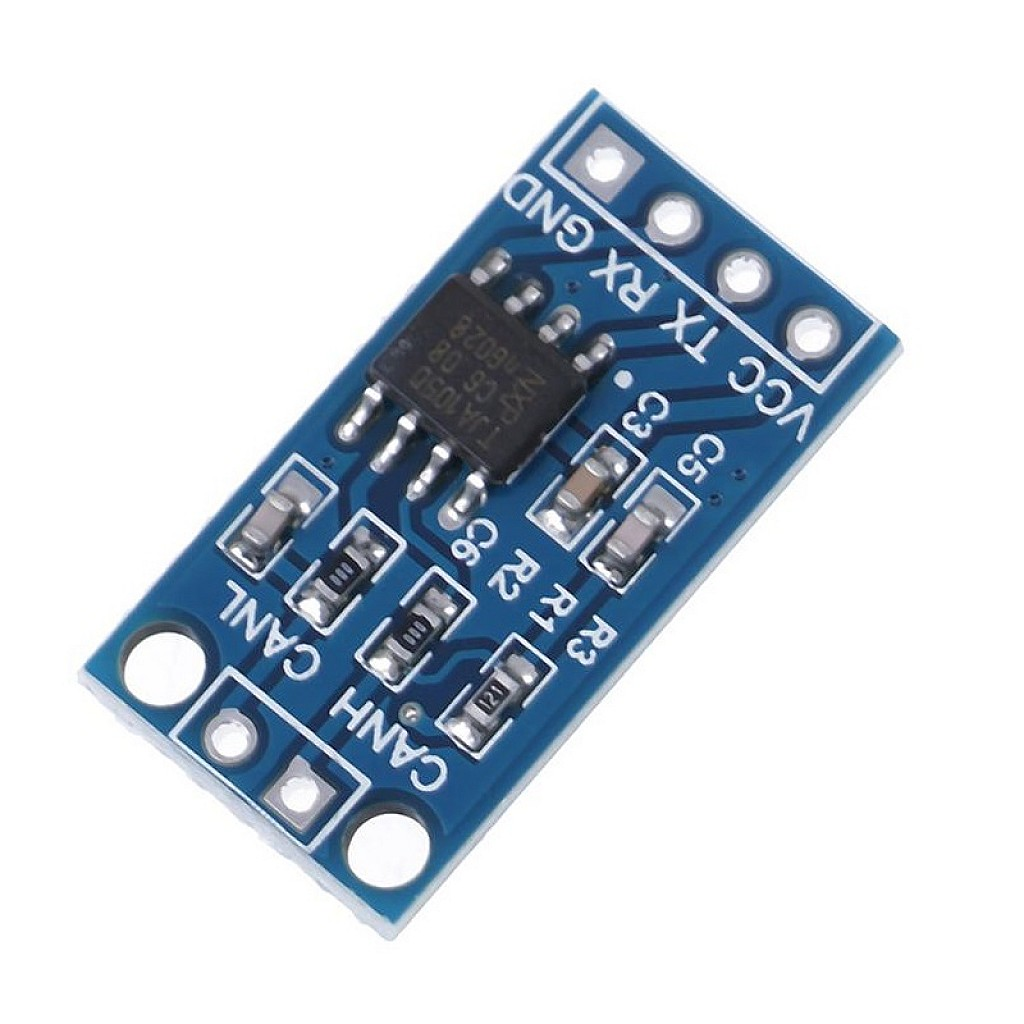
\includegraphics[width=0.5\textwidth]{images/TJA.png}
        \caption{Module CAN TJA1050}
    \end{figure}

\begin{table}[H]
\centering
\begin{tabular}{|>{\raggedright\arraybackslash}p{4.5cm}|>{\raggedright\arraybackslash}p{8.5cm}|}
\hline
\textbf{Thuộc tính} & \textbf{Mô tả} \\ \hline
Chuẩn giao tiếp & ISO 11898, CAN 2.0A/B \\ \hline
Điện áp cấp nguồn & 4,75 V -- 5,25 V (danh nghĩa 5 V) \\ \hline
Mức logic đầu vào & Tương thích 3,3 V và 5 V \\ \hline
Tốc độ tối đa & 1 Mbps \\ \hline
Chân kết nối chính & TXD, RXD, VCC, GND, CANH, CANL \\ \hline
Điện trở kết thúc bus & $120~\Omega$ tại mỗi đầu bus \\ \hline
\end{tabular}
\caption{Đặc điểm kỹ thuật của module TJA1050}
\end{table}

Một lưu ý quan trọng khi ghép ESP32 (3,3 V) với TJA1050 (5 V) là mức điện áp ngõ
ra của transceiver trả về GPIO của ESP32 có thể ở mức 5 V tùy phiên bản module.
Trong trường hợp này, cần sử dụng phân áp điện trở hoặc IC dịch mức logic để
bảo vệ vi điều khiển.

% ----------------------------------------------------------
\reportsubsection{5.1.3 Sơ đồ kết nối phần cứng}
% ----------------------------------------------------------

Sơ đồ kết nối giữa ESP32 và module TJA1050 được thể hiện trong Hình~5.1. Chân GPIO
26 của ESP32 làm đường truyền CAN logic, chân GPIO 27 làm đường nhận; hai chân này
nối trực tiếp tới các ngõ vào/ra tương ứng của transceiver. Từ transceiver, cặp
đường CANH/CANL đi ra bus chung

    \begin{figure}[H]
        \centering
        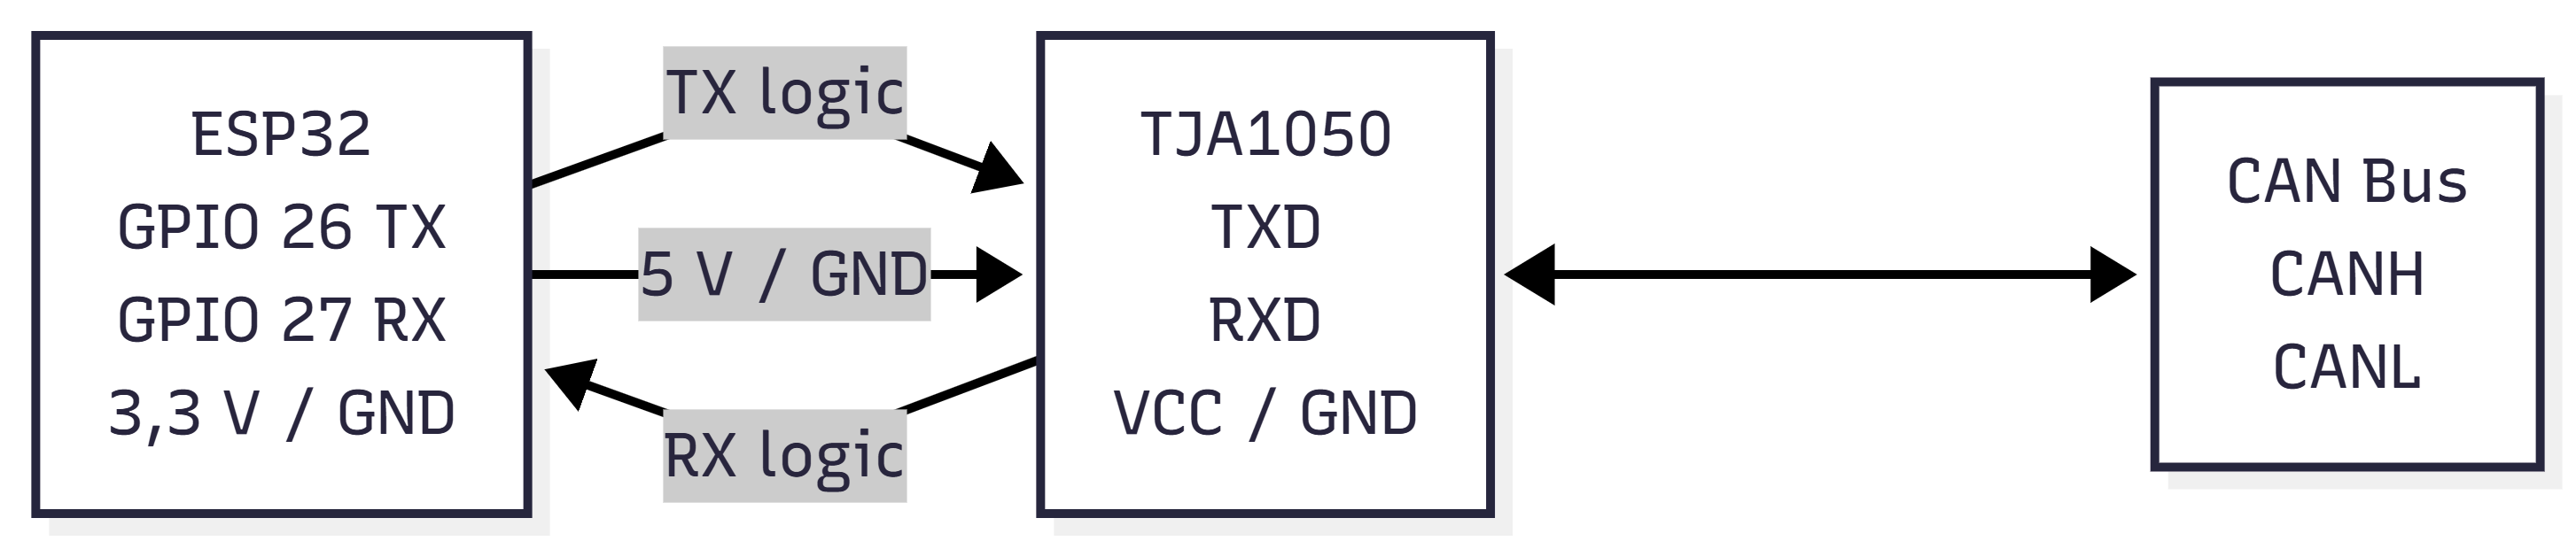
\includegraphics[width=0.85\textwidth]{images/so-do-ket-noi.png}
        \caption{Sơ đồ khối phần cứng tổng quan}
\end{figure}
% ============================================================
\reportsection{5.2 Hệ thống phần mềm}
% ============================================================

Hệ thống phần mềm được chia thành hai lớp phối hợp qua giao tiếp UART và
HTTP/WebSocket. Lớp thứ nhất là firmware nhúng chạy trực tiếp trên ESP32, chịu
trách nhiệm giao tiếp CAN, mô phỏng tấn công và phát hiện bất thường. Lớp thứ hai
là ứng dụng web chạy trên máy tính, đóng vai trò giao diện điều khiển và giám sát
thời gian thực. Kiến trúc tổng thể được mô tả trong Hình~5.3.

% ```mermaid
% graph TD
%     subgraph Firmware [Lớp Firmware ESP32]
%         direction LR
%         m1[Khởi động vòng lặp]
%         m2[Giao tiếp CAN]
%         m3[Terminal UART]
%         m4[Mô phỏng tấn công]
%         m5[Phát hiện xâm nhập]
%         m6[Ghi log]
%         m7[Quản lý trạng thái]
%         
%         m1 --> m2 & m3 & m4
%         m2 --> m5 & m6
%         m5 --> m7
%     end
%     
%     subgraph Web [Lớp Ứng dụng Web]
%         direction LR
%         w1[REST API]
%         w2[WebSocket]
%         w3[Mô phỏng phần mềm]
%         w4[Giao diện người dùng]
%         
%         w1 --> w2 --> w3
%     end
%     
%     m3 -. "UART 115.200 bps" .-> Web
%     Web -. "HTTP / WebSocket" .-> Firmware
% ```
\IfFileExists{images/kien-truc-phan-mem.png}{%
    \begin{figure}[H]
        \centering
        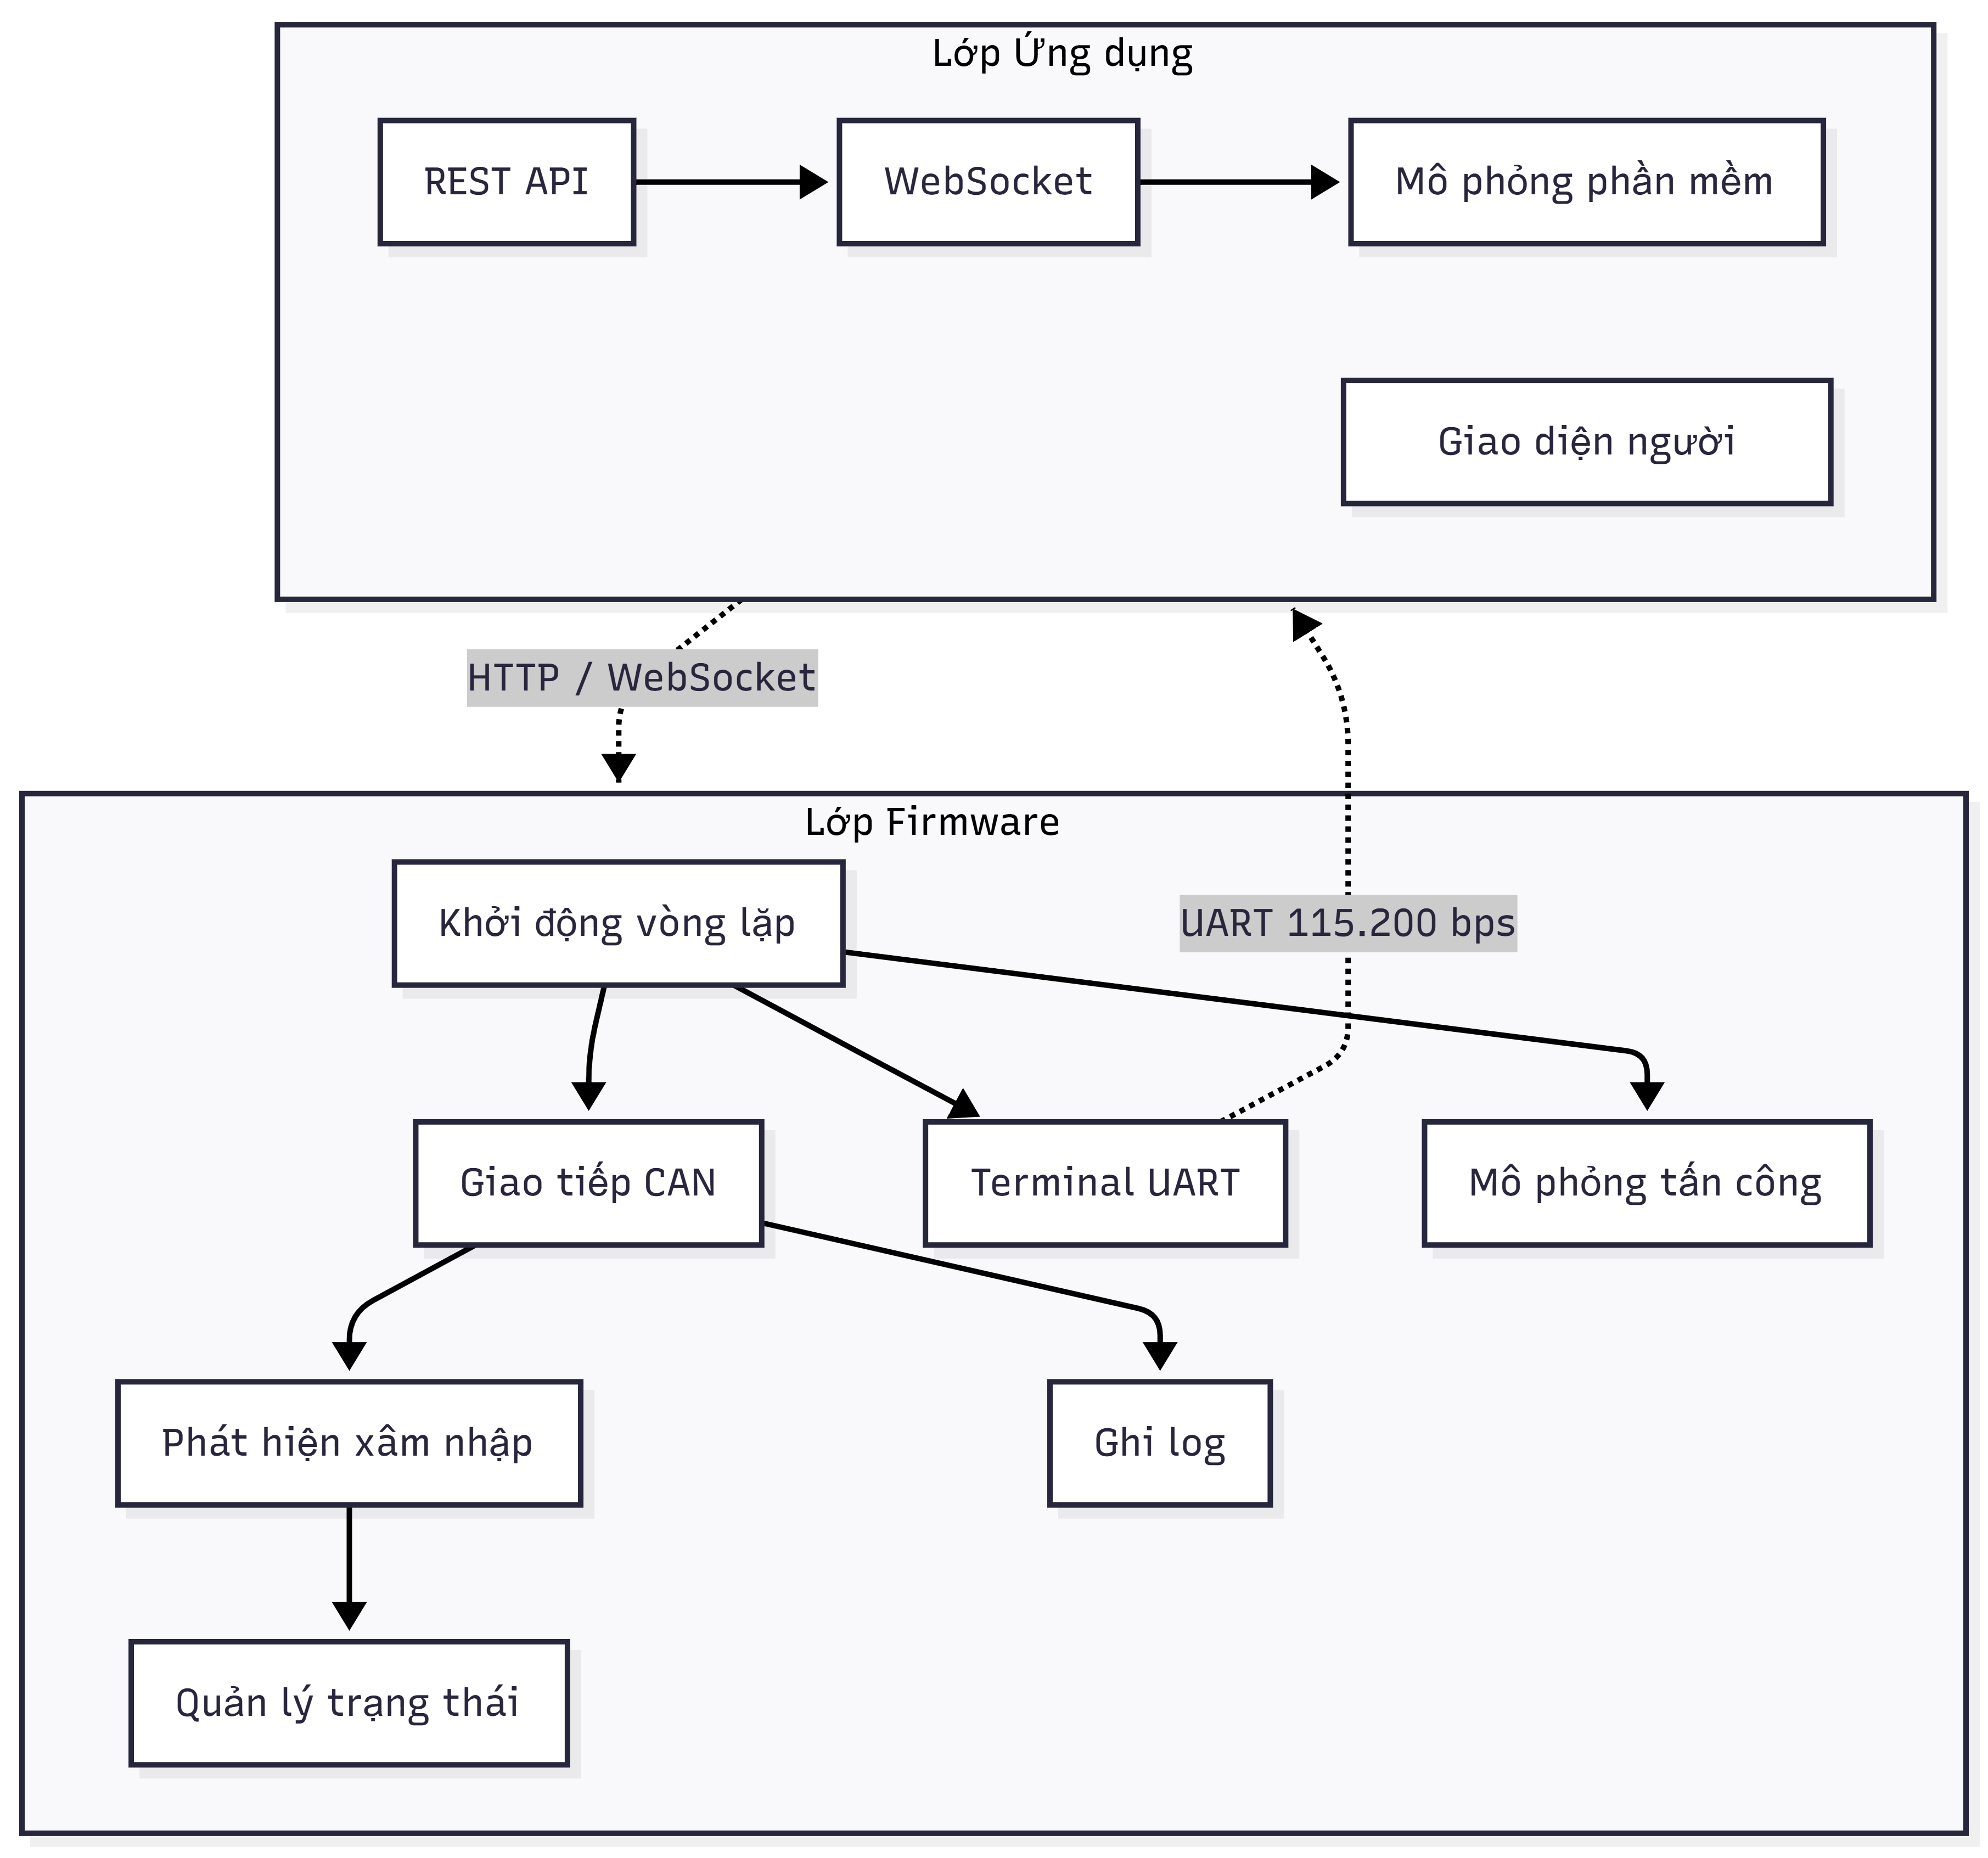
\includegraphics[width=0.85\textwidth]{images/kien-truc-phan-mem.png}
        \caption{Kiến trúc tổng thể hai lớp phần mềm của hệ thống}
    \end{figure}
}{%
    \IfFileExists{images/kien-truc-phan-mem.jpg}{%
        \begin{figure}[H]
            \centering
            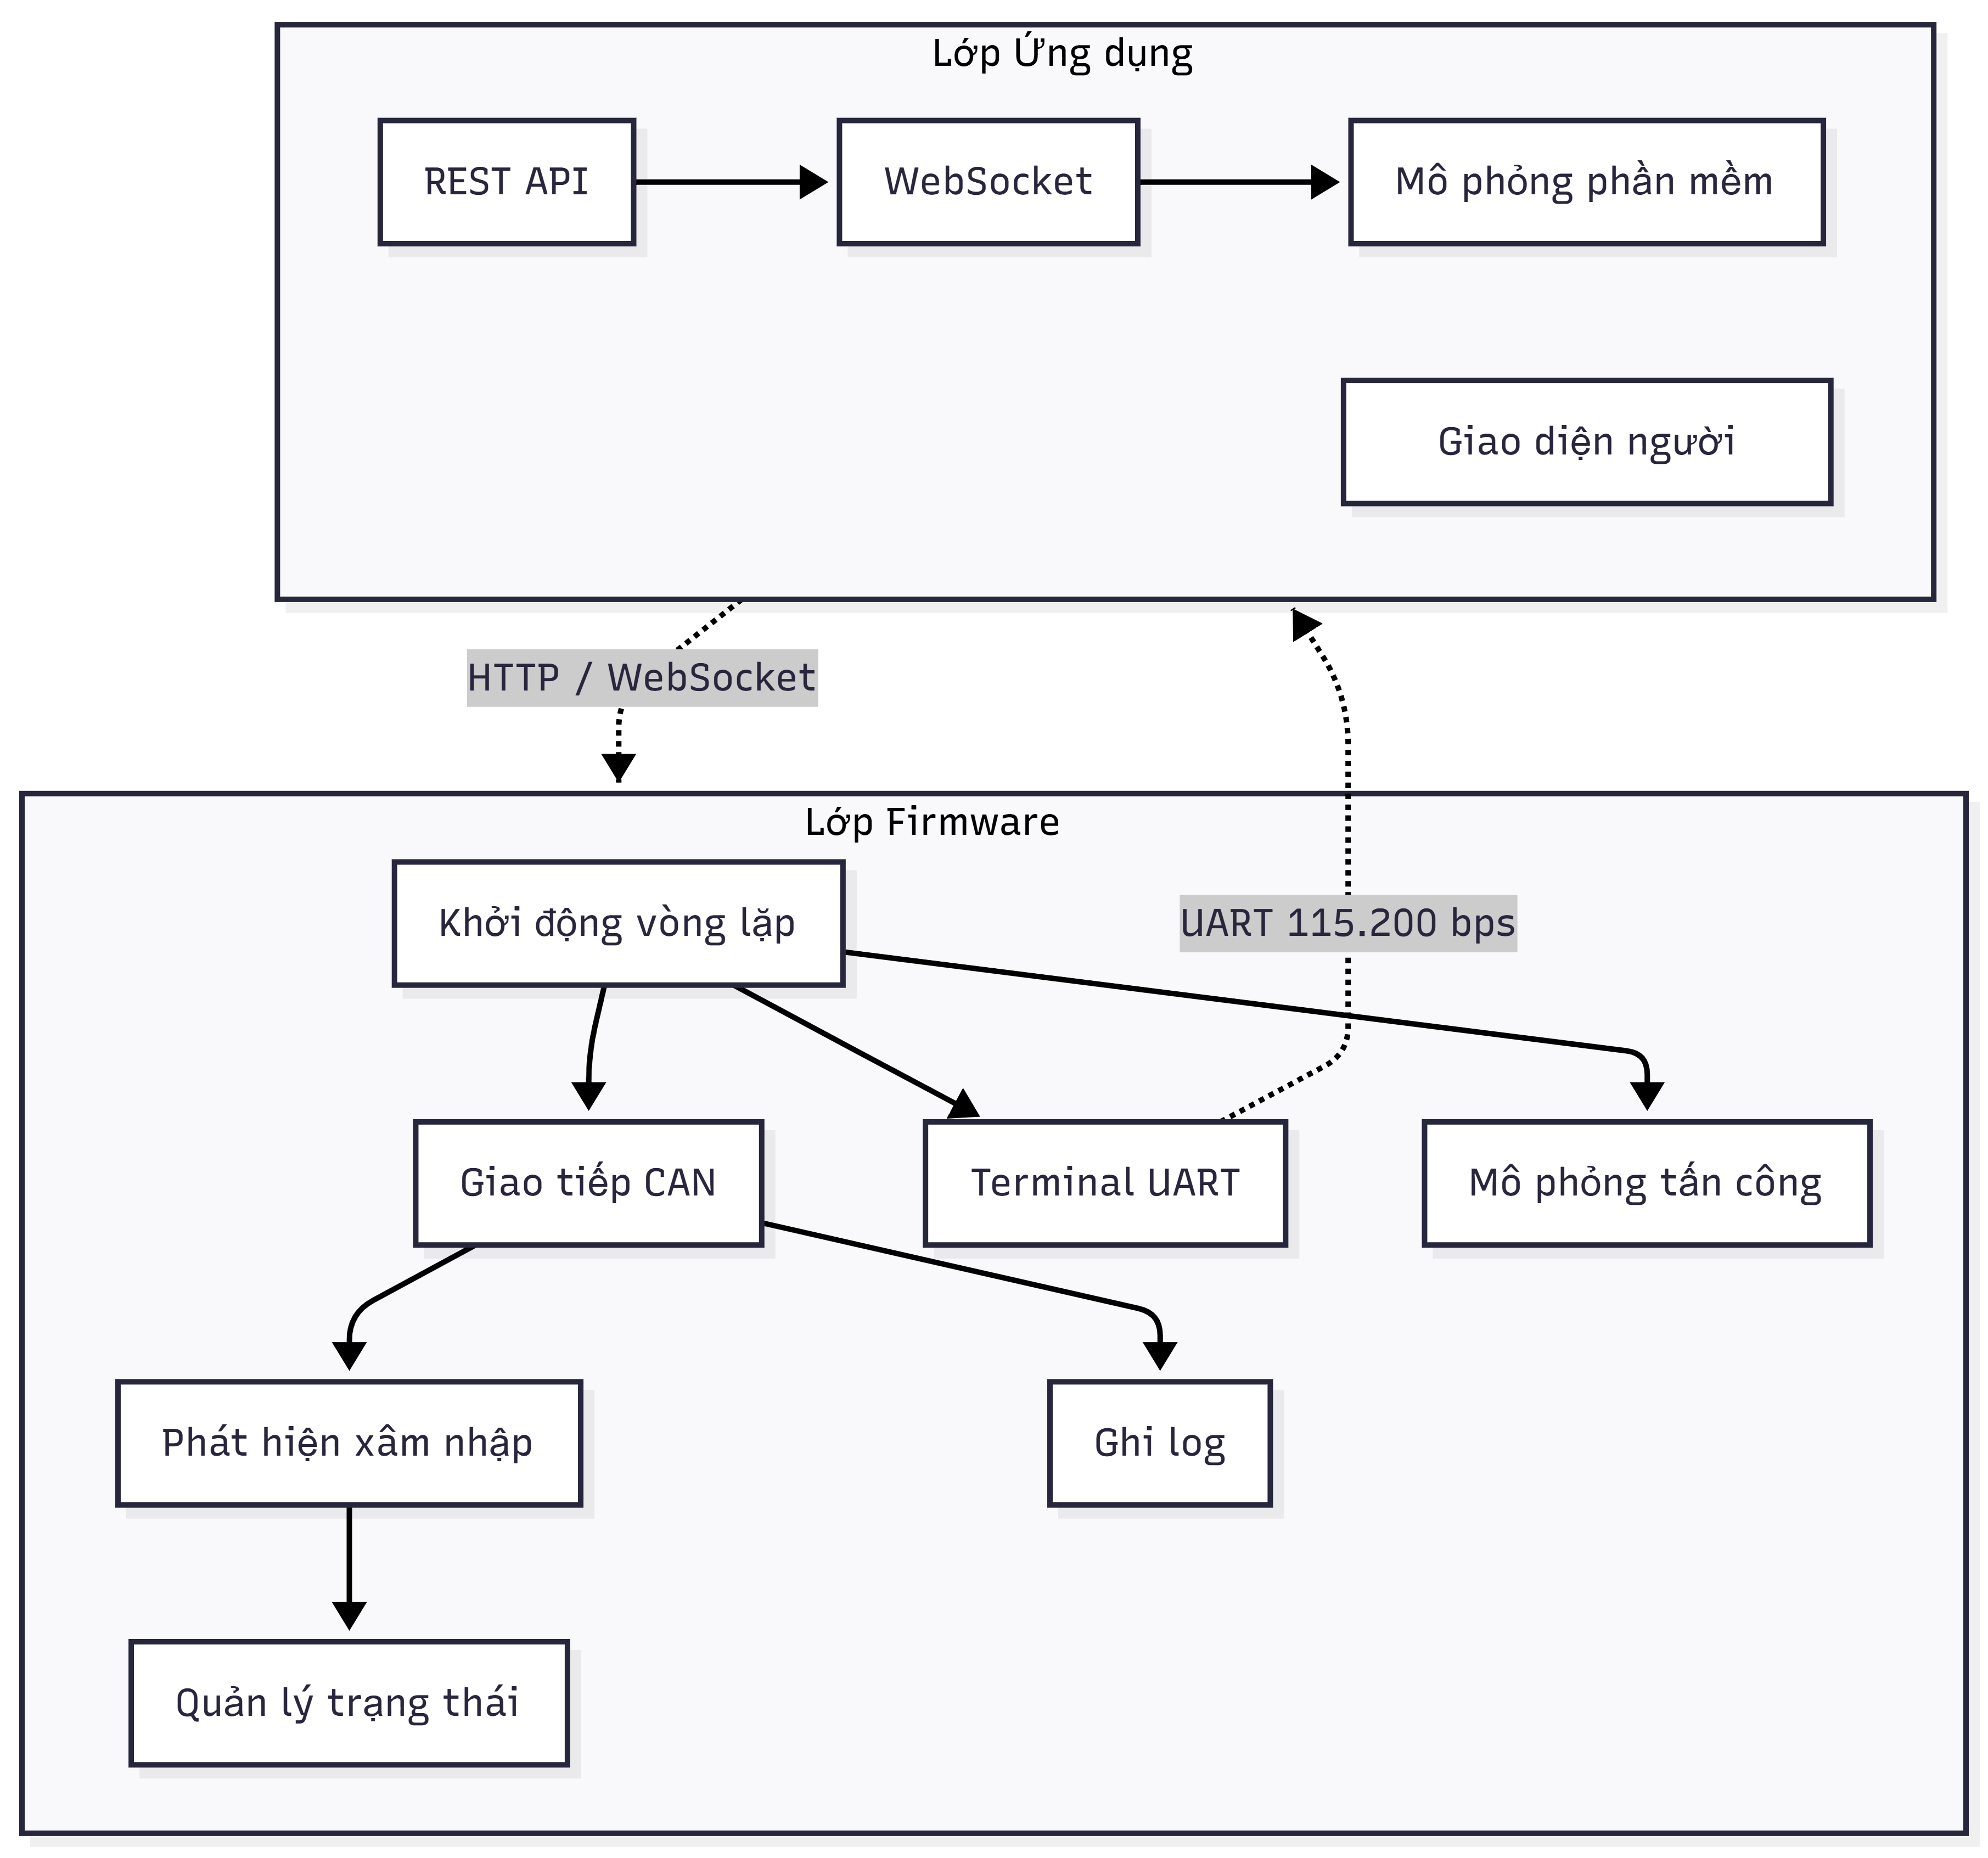
\includegraphics[width=0.85\textwidth]{images/kien-truc-phan-mem.jpg}
            \caption{Kiến trúc tổng thể hai lớp phần mềm của hệ thống}
        \end{figure}
    }{%
        \placeholderfigure{%
            Ảnh kiến trúc tổng thể hai lớp phần mềm của hệ thống.\\
            Đặt ảnh tại \texttt{report/images/kien-truc-phan-mem.png} hoặc \texttt{.jpg}%
        }{Kiến trúc tổng thể hai lớp phần mềm của hệ thống}
    }%
}

% ----------------------------------------------------------
\reportsubsection{5.2.1 Firmware ESP32}
% ----------------------------------------------------------

Firmware được tổ chức thành bảy mô-đun, mỗi mô-đun phụ trách một nhóm chức năng
độc lập. Các mô-đun giao tiếp với nhau qua một tập hợp biến trạng thái chia sẻ,
cho phép toàn bộ hệ thống hoạt động trong một luồng đơn mà không cần cơ chế đồng
bộ phức tạp.

\begin{table}[H]
\centering
\begin{tabular}{|>{\raggedright\arraybackslash}p{5cm}|>{\raggedright\arraybackslash}p{8.5cm}|}
\hline
\textbf{Mô-đun} & \textbf{Vai trò} \\ \hline
Khởi động và vòng lặp chính & Điều phối toàn bộ luồng xử lý của firmware \\ \hline
Giao tiếp CAN & Khởi tạo bus, gửi và nhận khung, bảo vệ bộ đếm \\ \hline
Xử lý lệnh terminal & Phân tích lệnh UART, in trạng thái hệ thống \\ \hline
Mô phỏng tấn công & Quản lý và thực thi năm loại tác vụ tấn công định kỳ \\ \hline
Phát hiện xâm nhập & Phân tích hành vi khung, sinh cảnh báo, quản lý luật chặn \\ \hline
Ghi log & Định dạng và xuất thông điệp ra UART theo chuẩn thống nhất \\ \hline
Quản lý trạng thái & Lưu trữ toàn bộ dữ liệu vận hành trong RAM nội bộ \\ \hline
\end{tabular}
\caption{Các mô-đun firmware và vai trò}
\end{table}

Các kiểu dữ liệu trung tâm được khai báo tập trung trong một tệp tiêu đề chung, bao
gồm cấu trúc khung CAN, bản ghi cảnh báo, khung được bắt gần nhất, các tác vụ tấn
công, bộ theo dõi từng ID và các cấu trúc phòng thủ. Nhờ đó, toàn bộ mô-đun chia
sẻ cùng một biểu diễn dữ liệu và giảm sự phụ thuộc lẫn nhau.

% ----------------------------------------------------------
\reportsubsection{5.2.2 Giao diện CAN và cơ chế bảo vệ bộ đếm}
% ----------------------------------------------------------

Mọi khung do người dùng tạo ra đều được kiểm tra và chuẩn hóa trước khi phát lên
bus. Quá trình này bao gồm: xác nhận CAN ID nằm trong phạm vi hợp lệ, kiểm tra độ
dài dữ liệu, và tự động chèn thêm một byte số thứ tự tăng dần vào cuối payload.
Nhờ đó, mỗi khung hợp lệ trên bus luôn mang một bộ đếm phân biệt giúp phát hiện
hành vi phát lại.

Ở phía nhận, mô-đun giao tiếp CAN đọc khung từ bus theo từng lô nhỏ. Mỗi khung
nhận được lần lượt qua các bước xử lý: kiểm tra xem ID có đang bị chặn bởi
cơ chế phòng thủ hay không, ghi log, phân tích bởi hệ thống phát hiện xâm nhập và
lưu lại làm khung bắt gần nhất để phục vụ tính năng replay.

% ----------------------------------------------------------
\reportsubsection{5.2.3 Hệ thống phát hiện xâm nhập (IDS)}
% ----------------------------------------------------------

Hệ thống phát hiện xâm nhập hoạt động theo hai cấp độ theo dõi song song. Ở cấp
độ đầu tiên, mỗi CAN ID trên bus được theo dõi riêng biệt bởi một bộ theo dõi
(tracker) lưu trữ lịch sử về tần suất xuất hiện, nội dung payload, bộ đếm thứ tự
và đường cơ sở bình thường. Hệ thống duy trì đồng thời tối đa 16 bộ theo dõi; khi
số ID vượt quá giới hạn, bộ theo dõi của ID ít hoạt động nhất sẽ được tái sử dụng.

Ở cấp độ thứ hai, một bộ theo dõi lưu lượng toàn cục quan sát hành vi tổng thể của
toàn bộ bus trong một cửa sổ thời gian trượt, ghi nhận số lượng ID mới và mức độ
thay đổi ID liên tiếp -- hai chỉ số đặc trưng của tấn công Fuzzing.

\begin{table}[H]
\centering
\begin{tabular}{|>{\raggedright\arraybackslash}p{3.6cm}|>{\raggedright\arraybackslash}p{3.8cm}|>{\raggedright\arraybackslash}p{6cm}|}
\hline
\textbf{Loại cảnh báo} & \textbf{Phương pháp phát hiện} & \textbf{Điều kiện kích hoạt} \\ \hline
Replay (phát lại) & So sánh bộ đếm & Byte số thứ tự không tăng đúng thứ tự \\ \hline
DoS (ngập lưu lượng) & Ước tính tốc độ & Tốc độ cùng ID $>$ 60 khung/giây \\ \hline
Fuzzing (quét ngẫu nhiên) & Theo dõi toàn bus & $\geq$ 4 ID mới, $\geq$ 5 đổi ID / 1,2 giây \\ \hline
Spoofing (giả mạo) & So sánh baseline & Payload lệch $\geq$ 2 byte so với mẫu bình thường \\ \hline
\end{tabular}
\caption{Tổng hợp các loại cảnh báo IDS và điều kiện kích hoạt}
\end{table}

% ----------------------------------------------------------
\reportsubsection{5.2.4 Bộ mô phỏng tấn công}
% ----------------------------------------------------------

Bộ mô phỏng tấn công cung cấp năm kiểu tấn công có thể kích hoạt độc lập qua
terminal UART hoặc giao diện web. Mỗi kiểu tấn công chạy như một tác vụ định kỳ
trong vòng lặp chính với chu kỳ có thể tùy chỉnh.

\begin{table}[H]
\centering
\begin{tabular}{|>{\raggedright\arraybackslash}p{2.5cm}|>{\raggedright\arraybackslash}p{2.5cm}|>{\raggedright\arraybackslash}p{8cm}|}
\hline
\textbf{Kiểu tấn công} & \textbf{Chu kỳ mặc định} & \textbf{Mô tả} \\ \hline
Replay & 250 ms & Phát lại nguyên bản khung hợp lệ đã bắt được, kể cả bộ đếm cũ \\ \hline
DoS & 20 ms & Ngập lưu lượng trên một CAN ID với tần suất cao \\ \hline
Fuzzing & 35 ms & Phát liên tục các khung với ID và payload ngẫu nhiên \\ \hline
Spoofing & 120 ms & Giả mạo ID của bản tin hợp lệ với nội dung bị biến đổi \\ \hline
\end{tabular}
\caption{Các kiểu tấn công được hỗ trợ}
\end{table}

Tấn công Replay có đặc điểm nổi bật là phát lại khung ở mức thô (wire level), tức
là không qua bước chuẩn hóa và bổ sung bộ đếm mới. Điều này khiến byte số thứ tự
bị lặp lại, tạo điều kiện cho IDS phát hiện. Tấn công Fuzzing sử dụng bộ sinh số
giả ngẫu nhiên để tạo ra các CAN ID và payload biến đổi liên tục trong mỗi chu kỳ.
Tấn công Spoofing dùng ID của một bản tin hợp lệ đã biết nhưng biến đổi nội dung
theo một mẫu xoay vòng qua từng chu kỳ phát.

% ----------------------------------------------------------
\reportsubsection{5.2.5 Ứng dụng web giám sát và điều khiển}
% ----------------------------------------------------------

Ứng dụng web sử dụng FastAPI làm backend và HTML/CSS/JavaScript thuần túy làm
giao diện người dùng. Hệ thống được khởi động dưới dạng máy chủ web tại cổng 8000,
phục vụ đồng thời giao diện HTML và luồng dữ liệu thời gian thực qua WebSocket.

Backend phân biệt hai chế độ kết nối nút. Trong chế độ phần cứng thực, backend
chuyển tiếp lệnh văn bản tới firmware qua cổng nối tiếp. Trong chế độ mô phỏng
phần mềm, backend tự sinh luồng sự kiện tấn công và phản hồi IDS mà không cần
phần cứng thực, phục vụ cho việc trình diễn giao diện. Giao diện web cung cấp đầy
đủ chức năng thêm/xóa nút, gửi khung CAN, kích hoạt từng kiểu tấn công và bật/tắt
cơ chế phòng thủ. Toàn bộ log và sự kiện được phát trực tiếp tới trình duyệt theo
thời gian thực qua kênh WebSocket.

% Gợi ý ảnh: chụp màn hình giao diện web đang hiển thị log và các nút điều khiển
% Đặt tại: report/images/web-interface.png hoặc .jpg
\IfFileExists{images/web-interface.png}{%
    \begin{figure}[H]
        \centering
        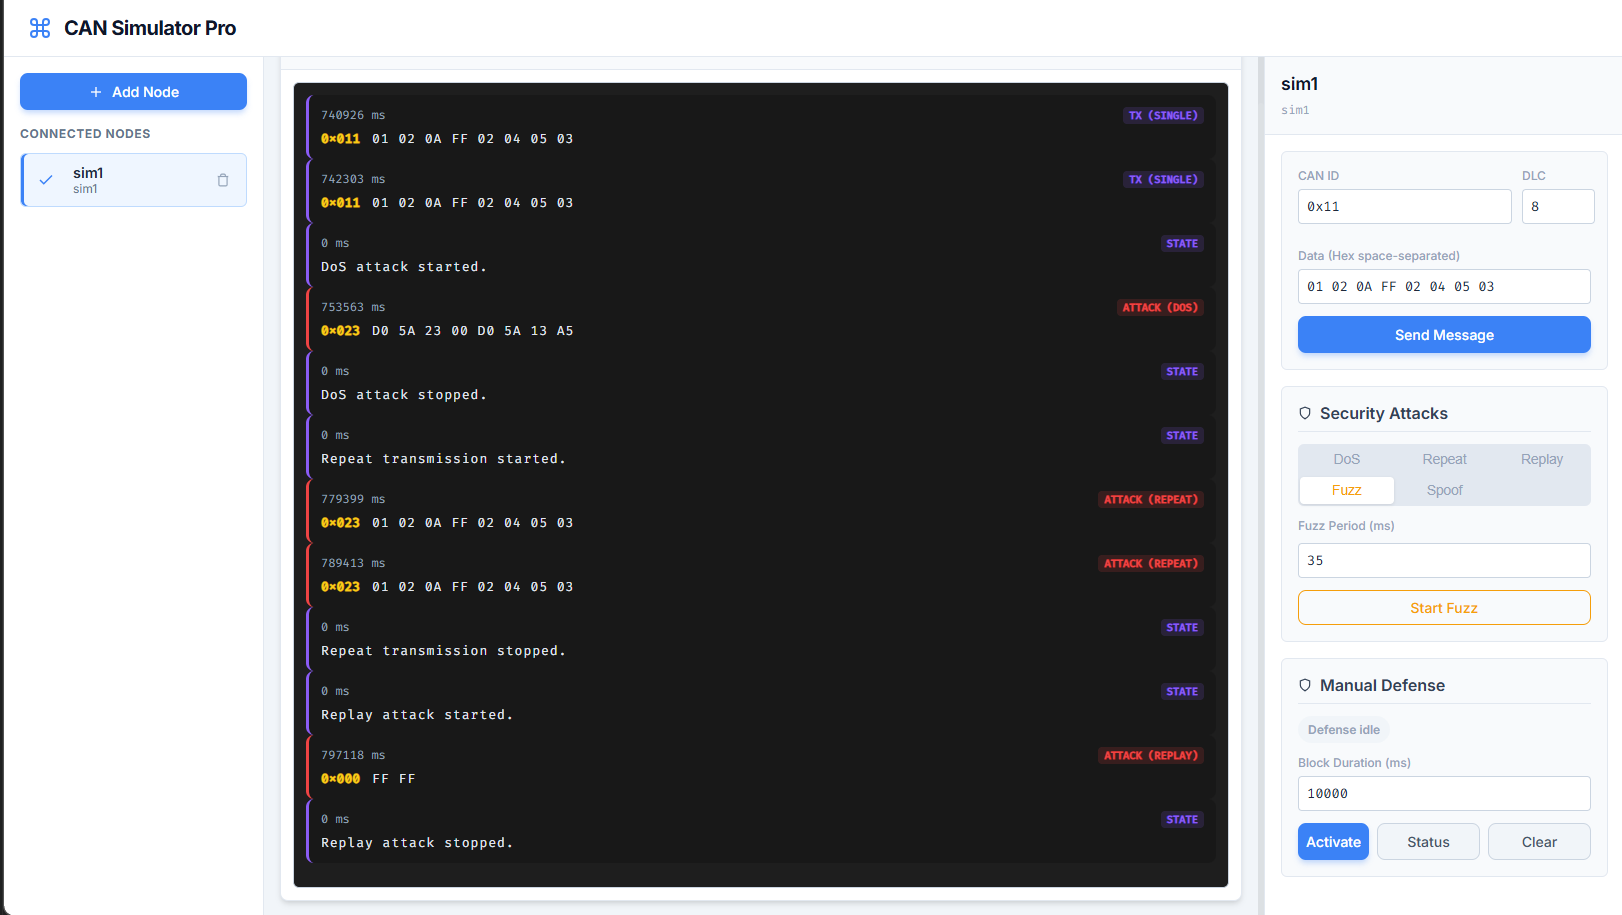
\includegraphics[width=0.88\textwidth]{images/web-interface.png}
        \caption{Giao diện web giám sát, tấn công và phòng thủ CAN}
    \end{figure}
}{%
    \IfFileExists{images/web-interface.jpg}{%
        \begin{figure}[H]
            \centering
            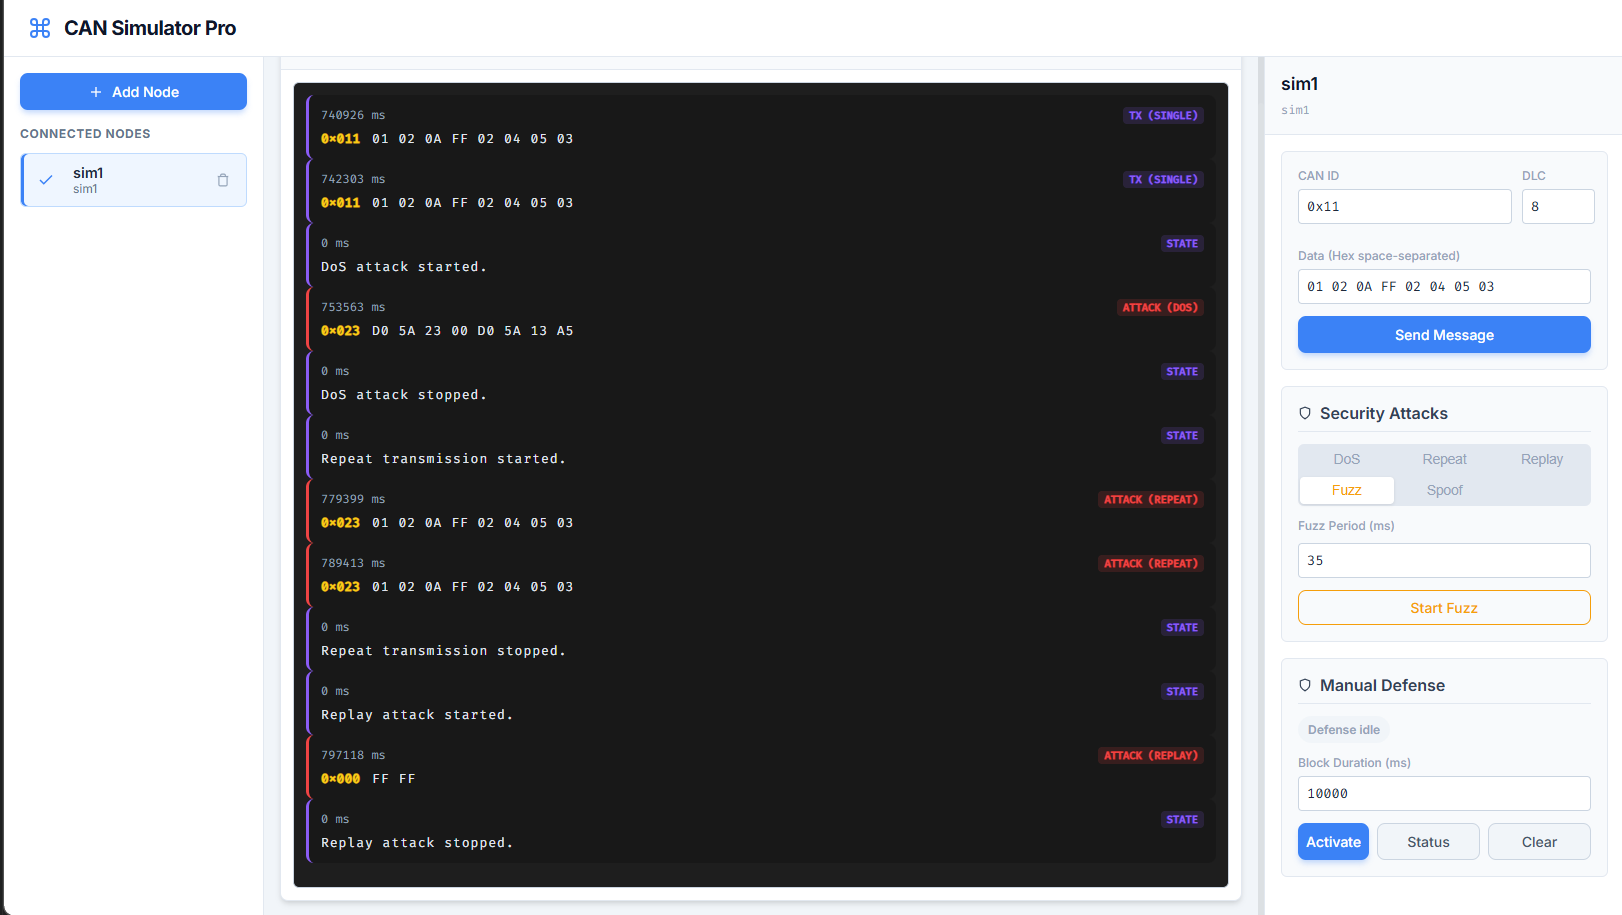
\includegraphics[width=0.88\textwidth]{images/web-interface.jpg}
            \caption{Giao diện web giám sát, tấn công và phòng thủ CAN}
        \end{figure}
    }{%
        \placeholderfigure{%
            Ảnh chụp màn hình giao diện web: danh sách nút, log thời gian thực,
            các nút kích hoạt tấn công và phòng thủ.\\
            Đặt ảnh tại \texttt{report/images/web-interface.png} hoặc \texttt{.jpg}%
        }{Giao diện web giám sát, tấn công và phòng thủ CAN}
    }%
}

% ----------------------------------------------------------
\reportsubsection{5.2.6 Quản lý trạng thái và lưu trữ dữ liệu}
% ----------------------------------------------------------

Hệ thống không sử dụng cơ sở dữ liệu lưu trữ bền vững. Phía firmware, toàn bộ
trạng thái vận hành được lưu trong bộ nhớ RAM nội bộ của ESP32, bao gồm khung bắt
gần nhất, bản ghi cảnh báo, các tác vụ tấn công đang chạy và bộ nhớ phòng thủ.
Dung lượng sử dụng nằm trong giới hạn an toàn của ESP32 với 520 kB SRAM tích hợp.

Phía ứng dụng web, trạng thái của tất cả nút và lịch sử khung quan sát được cũng
chỉ lưu trong bộ nhớ của tiến trình Python. Khi chương trình dừng, toàn bộ thông
tin này bị giải phóng. Thiết kế này phù hợp với mục tiêu trình diễn và thực nghiệm
ngắn hạn, nhưng cần bổ sung lớp lưu trữ bền vững nếu mở rộng sang các ứng dụng
giám sát dài hạn.

% ============================================================
\reportsection{5.3 Nguyên lý hoạt động của hệ thống}
% ============================================================

% ```mermaid
% flowchart TD
%     s1[Người dùng nhập lệnh terminal UART hoặc giao diện web]
%     s2[Kiểm tra ID, DLC và bổ sung byte số thứ tự]
% ```mermaid
% flowchart LR
%     s1("Nhập lệnh") --> s2("Chuẩn hóa") --> s3("Phát ra Bus")
%     s3 --> s4("Đọc từ Bus")
%     s4 --> d1{"Bị chặn?"}
%     
%     d1 -- "Có" --> drop("Loại bỏ")
%     d1 -- "Không" --> s5("Phân tích IDS")
%     
%     s5 -- "Phát hiện" --> alert("Sinh cảnh báo")
%     s5 -- "Bình thường" --> s6("Ghi log") --> s7("Cập nhật Web")
% ```
    \begin{figure}[H]
        \centering
        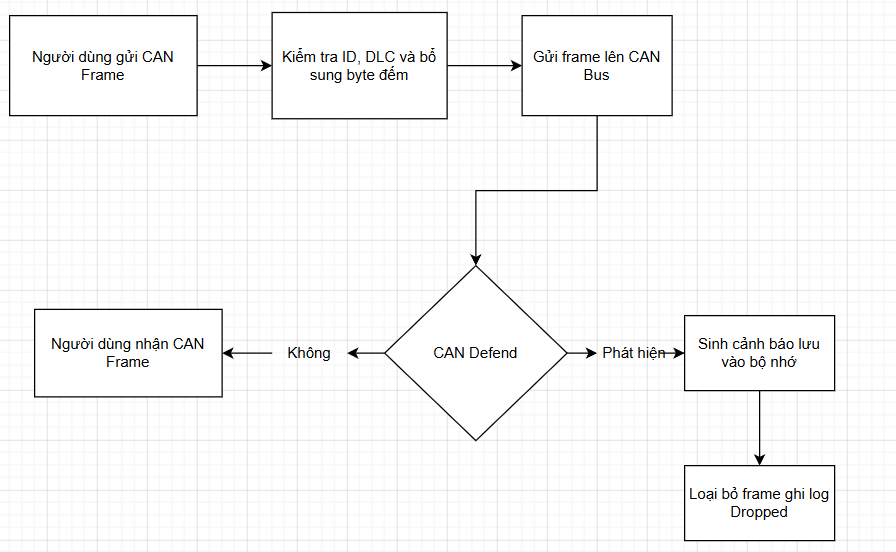
\includegraphics[width=0.75\textwidth]{images/so-do-luong-xu-ly.png}
        \caption{Sơ đồ luồng xử lý tổng thể của hệ thống}
    \end{figure}
%---------------------------------------------------------
\reportsubsection{5.3.1 Giao tiếp CAN cơ bản}
% ----------------------------------------------------------

Ở chế độ bình thường, người dùng gửi một khung CAN đơn bằng lệnh
\texttt{send <id> <dlc> <data>} qua terminal. Firmware kiểm tra tính hợp lệ của
các tham số, bổ sung byte số thứ tự vào cuối payload rồi phát lên bus. Khi nhận
được khung từ bus, nút ghi log theo định dạng chuẩn có nhãn thời gian, chiều
truyền, CAN ID, độ dài dữ liệu và nội dung. Đồng thời khung được lưu lại làm dữ
liệu nền cho tính năng phát lại. LED trên bo mạch nhấp nháy ngắn để xác nhận mỗi
sự kiện truyền hoặc nhận thành công.

% ----------------------------------------------------------
\reportsubsection{5.3.2 Cơ chế bảo vệ bộ đếm thông điệp}
% ----------------------------------------------------------

Khi tính năng bảo vệ bộ đếm được bật, mỗi khung gửi đi đều có thêm một byte số
thứ tự tăng dần ở vị trí byte cuối cùng của payload, làm tổng độ dài tăng lên một
byte. Bộ đếm là số nguyên 8-bit không dấu, tăng liên tục và quay về 0 sau giá trị
255. Phía nhận đọc byte cuối của mỗi khung đến, đối chiếu với giá trị kỳ vọng dựa
trên lần nhận trước của cùng CAN ID. Bất kỳ sai lệch nào đều bị ghi nhận là dấu
hiệu bất thường và sinh cảnh báo phát lại loại đếm ngược.

% ----------------------------------------------------------
\reportsubsection{5.3.3 Replay Attack}
% ----------------------------------------------------------

\begin{itemize}[leftmargin=*]
    \item \textbf{Mô hình tấn công:} Tấn công phát lại (Replay Attack) xảy ra khi một thực thể trái phép tiến hành rình rập (sniffing) và sao chép các thông điệp CAN hợp lệ đang truyền tải trên bus. Sau đó, thực thể này tái phát (inject) các thông điệp nguyên bản đó vào mạng tại một thời điểm khác.
    \item \textbf{Hậu quả:} Các Bộ điều khiển điện tử (ECU) sẽ tiếp nhận và thực thi các lệnh bị lặp lại (ví dụ: kích hoạt hệ thống phanh, vô hiệu hóa khóa cửa) do giao thức CAN nguyên thủy thiếu vẹn toàn về nhãn thời gian. Điều này dẫn đến sự sai lệch nghiêm trọng trong trạng thái vận hành của phương tiện.
    \item \textbf{Cơ chế phòng thủ:} Giải pháp lý thuyết tối ưu để ngăn chặn tấn công phát lại là tích hợp các định danh động như bộ đếm tăng dần (Monotonic Counter) hoặc Mã xác thực thông điệp (MAC) vào dữ liệu tải. Qua đó, hệ thống phát hiện xâm nhập (IDS) có thể kiểm chứng tính mới (freshness) của dữ liệu và loại bỏ các gói tin lỗi thời.
\end{itemize}



% ----------------------------------------------------------
\reportsubsection{5.3.4 Spoofing Attack}
% ----------------------------------------------------------

\begin{itemize}[leftmargin=*]
    \item \textbf{Mô hình tấn công:} Tấn công giả mạo (Spoofing) là kỹ thuật đánh lừa định tuyến, trong đó kẻ tấn công phát đi các khung dữ liệu mang CAN ID hợp lệ nhưng cố ý ngụy tạo cấu trúc hoặc giá trị của vùng dữ liệu tải (payload) nhằm đánh lừa các ECU đích.
    \item \textbf{Hậu quả:} Việc tiêm các thông số giả mạo (ví dụ: tốc độ vòng tua động cơ, nhiệt độ cảm biến) sẽ làm nhiễu loạn logic điều khiển của hệ thống. Nếu các ECU đưa ra quyết định dựa trên luồng dữ liệu giả mạo này, sự an toàn cơ học của phương tiện có thể bị đe dọa trực tiếp.
    \item \textbf{Cơ chế phòng thủ:} Phương thức phòng vệ nền tảng là xây dựng mô hình hành vi bình thường (baseline) cho mạng CAN dựa trên chu kỳ phát và đặc trưng tải trọng của từng định danh. Mọi sự sai lệch bất thường về độ dài dữ liệu (DLC) hoặc giá trị payload lệch khỏi quỹ đạo thống kê đều bị IDS phân loại là hành vi giả mạo.
\end{itemize}

% ----------------------------------------------------------
\reportsubsection{5.3.5 DoS Attack}
% ----------------------------------------------------------

\begin{itemize}[leftmargin=*]
    \item \textbf{Mô hình tấn công:} Tấn công từ chối dịch vụ (Denial of Service - DoS) được thực thi thông qua việc bơm tràn ngập (flooding) mạng CAN bằng các khung dữ liệu mang định danh có mức độ ưu tiên cao nhất (CAN ID mang giá trị thấp) với tần suất cực đại.
    \item \textbf{Hậu quả:} Do cơ chế phân xử tranh chấp dựa trên mức ưu tiên (Arbitration) của giao thức CAN, các thông điệp từ các ECU hợp lệ sẽ liên tục bị từ chối quyền truy cập bus. Trạng thái này gây ra độ trễ nghiêm trọng hoặc làm tê liệt hoàn toàn khả năng trao đổi thông tin của toàn mạng.
    \item \textbf{Cơ chế phòng thủ:} Cơ sở lý luận để giảm thiểu DoS là giám sát và phân tích lưu lượng dựa trên tần suất (Rate-based Intrusion Detection). Hệ thống IDS cần tính toán mật độ thông điệp trong các cửa sổ thời gian (time windows). Bất cứ nút nào phát sinh lưu lượng vượt quá giới hạn băng thông lý thuyết của mạng sẽ bị nhận diện và cách ly.
\end{itemize}



% ----------------------------------------------------------
\reportsubsection{5.3.6 Fuzzing Attack}
% ----------------------------------------------------------

\begin{itemize}[leftmargin=*]
    \item \textbf{Mô hình tấn công:} Quét ngẫu nhiên (Fuzzing) là chiến lược tấn công diện rộng, trong đó kẻ tấn công liên tục tiêm vào bus hàng loạt khung CAN với các định danh (ID) và vùng dữ liệu tải (payload) được sinh ngẫu nhiên hoàn toàn sau mỗi chu kỳ.
    \item \textbf{Hậu quả:} Cuộc tấn công này đẩy các ECU vào trạng thái phải liên tục xử lý một khối lượng khổng lồ các thông điệp rác không xác định. Việc này không chỉ gây lãng phí tài nguyên xử lý mà còn có thể vô tình kích hoạt các chức năng ẩn (diagnostic messages), dẫn đến hệ thống hoạt động hỗn loạn.
    \item \textbf{Cơ chế phòng thủ:} Khác với việc giám sát theo từng ID đơn lẻ, nguyên lý nhận diện Fuzzing dựa trên phép phân tích tính biến động toàn cục của bus. Sự xuất hiện ồ ạt của các ID ngoại lai hoặc tỷ lệ luân chuyển ID quá cao trong một đơn vị thời gian là các đặc trưng dị thường giúp IDS kích hoạt trạng thái phòng vệ.
\end{itemize}



% ----------------------------------------------------------
\reportsubsection{5.3.7 Cơ chế phòng thủ chủ động}
% ----------------------------------------------------------

Sau khi IDS phát sinh cảnh báo, người vận hành có thể kích hoạt phòng thủ qua lệnh
terminal hoặc nút tương ứng trên giao diện web. Hệ thống đọc thông tin từ cảnh báo
gần nhất và thiết lập quy tắc chặn phù hợp với từng loại tấn công. Thời gian
duy trì luật chặn mặc định là 10 giây nhưng có thể tùy chỉnh.

\begin{table}[H]
\centering
\begin{tabular}{|>{\raggedright\arraybackslash}p{3.2cm}|>{\raggedright\arraybackslash}p{4.0cm}|>{\raggedright\arraybackslash}p{6.2cm}|}
\hline
\textbf{Loại tấn công} & \textbf{Đối tượng bị chặn} & \textbf{Tiêu chí lọc} \\ \hline
Replay (phát lại) & Khung cùng ID và nội dung & Khớp chính xác với chữ ký khung bị cảnh báo \\ \hline
DoS (ngập lưu lượng) & Mọi khung cùng ID & Chặn toàn bộ, không phân biệt nội dung \\ \hline
Spoofing (giả mạo) & Khung cùng ID đáng ngờ & Lọc theo độ lệch so với baseline đã học \\ \hline
Fuzzing (quét ngẫu nhiên) & Mọi ID chưa tin cậy & Chỉ cho phép ID đã ổn định trước cảnh báo \\ \hline
\end{tabular}
\caption{Chiến lược phòng thủ theo từng loại tấn công}
\end{table}

Cần lưu ý rằng cơ chế phòng thủ hiện tại hoạt động ở tầng phần mềm của nút nhận,
không loại bỏ khung tấn công khỏi bus vật lý. Kẻ tấn công vẫn có thể tiếp tục phát
khung; hệ thống chỉ ngăn tầng ứng dụng xử lý các khung bị nghi ngờ trong thời gian
áp dụng luật chặn. Đây là hạn chế vốn có của kiến trúc CAN không có cơ chế xác thực ở lớp
liên kết dữ liệu và là hướng mở rộng tiếp theo của đề tài.
